% This file was created by tikzplotlib v0.9.8.
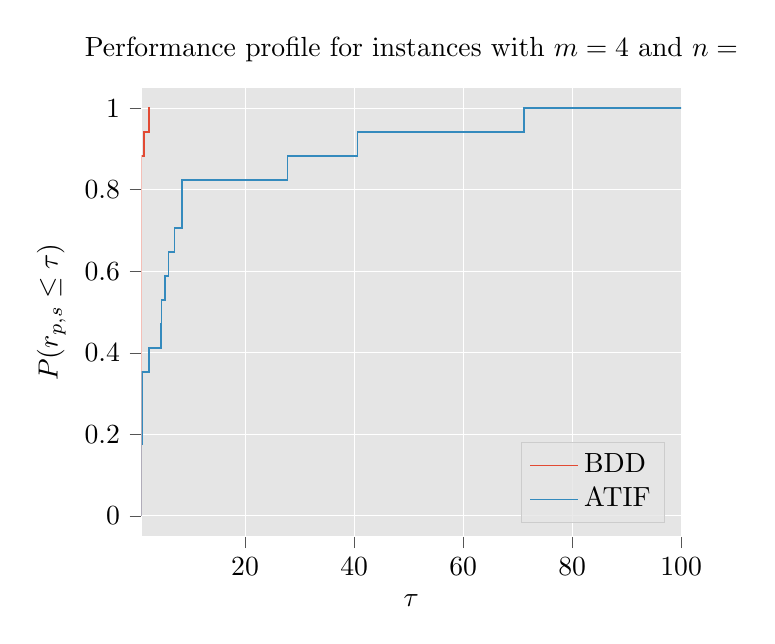
\begin{tikzpicture}

\definecolor{color0}{rgb}{0.886274509803922,0.290196078431373,0.2}
\definecolor{color1}{rgb}{0.203921568627451,0.541176470588235,0.741176470588235}

\begin{axis}[
axis background/.style={fill=white!89.8039215686275!black},
axis line style={white},
legend cell align={left},
legend style={
  fill opacity=0.8,
  draw opacity=1,
  text opacity=1,
  at={(0.97,0.03)},
  anchor=south east,
  draw=white!80!black,
  fill=white!89.8039215686275!black
},
tick align=outside,
tick pos=left,
title={Performance profile for instances with \(\displaystyle m = 4\) and \(\displaystyle n = \)},
x grid style={white},
xlabel={\(\displaystyle \tau\)},
xmajorgrids,
xmin=1, xmax=100,
xtick style={color=white!33.3333333333333!black},
y grid style={white},
ylabel={\(\displaystyle P(r_{p,s} \leq \tau)\)},
ymajorgrids,
ymin=-0.05, ymax=1.05,
ytick style={color=white!33.3333333333333!black}
]
\addplot [semithick, color0, const plot mark right]
table {%
1 0
1 0.0588235294117647
1 0.117647058823529
1 0.176470588235294
1 0.235294117647059
1 0.294117647058824
1 0.352941176470588
1 0.411764705882353
1 0.470588235294118
1 0.529411764705882
1 0.588235294117647
1 0.647058823529412
1 0.705882352941177
1 0.764705882352941
1 0.823529411764706
1.51500864433759 0.882352941176471
2.43099124624187 0.941176470588235
2.44140598848904 1
};
\addlegendentry{BDD}
\addplot [semithick, color1, const plot mark right]
table {%
1 0
1 0.0588235294117647
1 0.117647058823529
1.04685068286893 0.176470588235294
1.06120665510274 0.235294117647059
1.13911930064946 0.294117647058824
2.40805178965669 0.352941176470588
4.57353594785599 0.411764705882353
4.6356844369852 0.470588235294118
5.36212721294338 0.529411764705882
5.97507706508315 0.588235294117647
7.02957927761404 0.647058823529412
8.42459346795663 0.705882352941177
8.45252282092818 0.764705882352941
27.7517962642493 0.823529411764706
40.6084498500117 0.882352941176471
71.162049784891 0.941176470588235
424.735217558257 1
};
\addlegendentry{ATIF}
\end{axis}

\end{tikzpicture}
